
%----------------------------------------------------------------------------------------------------------------------------------------

% définit le type de document et ses options
\documentclass[a4paper,10pt]{article}

% des paquetages indispensables, qui ajoutent des fonctionnalités
\usepackage[utf8]{inputenc}
\usepackage{graphicx}
\usepackage{lscape}
\usepackage{url}
\usepackage{xspace}
\usepackage[francais]{babel}
\usepackage{fullpage}

\pagestyle{plain}


%----------------------------------------------------------------------------------------------------------------------------------------


% le debut du contenu
\begin{document}


%----------------------------------------------------------------------------------------------------------------------------------------


%%%%%%%%%%%%%%%%%%%%%%%%%%%%%%%%%%%%%%%%%%%%%%%%%
%%Page d'accueil
\begin{center}
	%%
	\hspace{3cm}
	
\includegraphics[scale=0.8]{logo.ps}

	%%
	\vspace{1cm}
	{\large Projet de spécialité 2010}\\
	{\Large Conception d'un modèle de feu 3D temps réel}\\
	\vspace{1cm}


	\includegraphics[scale=0.3]{feu.ps}\\
	\vspace{2cm}
	%%
	Étudiants impliqués :\\
	Benjamin Aupetit - IRVM - benjamin.aupetit@ensimag.imag.fr\\
	Julien Champeau - IRVM - julien.champeau@ensimag.imag.fr\\
	Arnaud Emilien - IRVM - arnaud.emilien@ensimag.imag.fr\\
	~\\
	Encadrants :\\
	Marie-Paule Cani  -  Marie-Paule.Cani@inrialpes.fr \\
	Aurélie Catel - aurelie.catel@grenoble-inp.fr
	~ \\
	\vspace{3mm}
	Ensimag 2010\\

\end{center}


\newpage

\tableofcontents

\newpage



%----------------------------------------------------------------------------------------------------------------------------------------
%%%%%%%%%%%%%%%%%
\section{Présentation du projet}
\subsection{Introduction}
Il existe de nombreux travaux de modélisation du feu. Cependant, peu d'entre eux
modélisent la totalité du processus de combustion. Nous avons trouvé interessant
de répondre à la problématique : comment modéliser une combustion réaliste et temps réel?


\subsection{Objectifs initiaux}
Le but principal de notre projet est de réaliser un modèle de combustion en 3D temps
réel. \\
Cette modélisation devra être la plus réaliste possible : en
effet nous voulons permettre d'intégrer notre solution dans un
environnement temps réel qui requiert un comportement proche de la
réalité en restant interactif.
Dans ce sens notre solution ne sera pas adaptée à tous les jeux vidéos, car ceux ci ne nécessitent pas une
approche réaliste mais juste des effets visuels impressionnants.\\

Notre solution devra ainsi répondre aux critères suivants :
\begin{itemize}
\item Modèle de flamme convainquant. 
\item Génération de fumée.
\item Propagation réaliste sur l'objet. 
\item Prise en compte des flux d'air ( vent, advection du feu... )
\item Interaction du système avec les objets.
\item Destruction procédurale progressive d'un objet.
\item Propagation à l'environnement.\\
\end{itemize}


\subsection{Moyens utilisés}
Sachant que nous voulons réaliser une application temps réel, nous avons décider dans 
un premier temps de le réaliser sur \textbf{CPU} en utilisant \textbf{OpenGL} pour valider le modèle, 
puis de l'adapter en \textbf{Shader GLSL}. Les calculs réalisés étant hautement 
parallélisables, la programmation sur GPU est indispensable.

\subsection{La démarche}
Notre démarche a été similaire à celle d'un chercheur effectuant une nouvelle
publication. En effet, nous avons commencé par effectuer une série de recherche
bibliographique pour saisir au mieux les avantages et inconvénients de différentes
méthodes, et ainsi d'en tirer le meilleur pour réaliser notre modèle.\\
Nous avons effectué un compte rendu de la plupart des articles lu, ceux-ci
se trouvent dans la partie \textbf{recherche bibliographique} de ce document.\\
Nous avons ensuite implémenté notre modèle dont nous justifions les choix
dans la suite de ce document.


\subsection{Résultats}
Nous avons ainsi implémenté totalement le modèle de fluide et d'objet sur CPU, 
et le modèle de fluide sur GPU. Le modèle d'objet nécessite une adaptation plus
importante aux fonctionalités de la carte graphique, que nous expliquerons 
dans la suite de ce document.\\
Le modèle CPU présente un taux d'image par secondes suffisant pour montrer 
le bon fonctionnement du modèle. Toutes les fonctionalités du modèles sont
implémentées et opérationelles. (environ 9 fps avec une grille 40x40x40)\\
La version GPU est comme prévu beaucoup plus rapide et permet d'utiliser
une taille de grille plus importante. (environ 9 fps avec une grille 100x100x100)\\
Nous avons donc réussi à optenir un modèle de combustion complet et intéractif en CPU,
et un modèle de fluide complet en GPU. L'ajout d'un modèle 
d'objet au GPU de devrait pas trop affecter les performances. Les performances sont 
donc suffisamment bonnes pour valider notre contrainte de temps réel.



%%%%%%%%%%%%%%%%%
\section{Aperçu de notre modèle}
Ici nous présentons un résumé de notre modèle global. Ce modèle a été
établi pour unifier les différents modèles du processus de combustion. 
En effet nous devons nous assurer de la compatibilité de ceux ci, pour éviter les incohérences entre les
différentes étapes, ou des calculs de synchronisation entre les
phases. 

\subsection{Les flammes}
Pour modéliser les flammes il faut différencier deux aspects. Le rendu
des flammes d'une part, et la modélisation du phénomène associé
d'autre part.

\subsubsection{Un modèle de fluide pour le feu}
Le modèle de fluide est basé sur les travaux de \textbf{Jos Stam, stable fluids}. 
Ce modèle inclue la diffusion de la densité de gaz, la densité de fumée, la chaleur, 
la vitesse de l' air. Il permet aussi de gérer plus
simplement la diffusion du feu entre les objets dans tout son environnement.

\subsubsection{Le rendu des flammes et de la fumée}
Pour rendre les flammes nous avons besoin d'une méthode rapide mais
donnant une impression de réalisme. Pour faire ceci nous utilisons une
méthode inspirée de celle de \textbf{Zeki Melek}. Notre méthode consiste à
transformer la matrice du fluide en texture3D, puis de découper le fluide en 
``tranches'' orthogonales à l'orientation de la camera. Pour chaque tranche,
nous calculons les coordonnées de textures des points la constituant. 
Ainsi notre méthode de \textbf{rendu de texture3D} permet de visualiser le fluide
à 360 degrés.\\
Nous utilisons de plus un shader GLSL de \textbf{multitexturing}. Ce shader
permet dans un premier temps de choisir si nous devons afficher la flamme ou la
fumée, en fonction qui rajoute un \textbf{bruit de Perlin}
aux coordonnées de texture, multiplié par un \textbf{dégradé vertical}. Ceci
permet d'avoir une flamme réaliste, dont les flammes sont plus violentes
dessus que dessous.\\
Enfin, nous déterminons la couleur de la flamme en nous basant sur le
\textbf{principe du corps noir}, qui détermine la coloration de la flamme
en fonction de la chaleur.

\subsection{Les objets}
\subsubsection{L'ajout des objets au modèle de fluide}
Nos objets sont représentés sous formes de \textbf{grilles de voxels}, ce qui 
permet d'interagir facilement avec la grille uniforme du fluide.
Ces grilles de voxels sont indépendantes du fluide, et propres à chaque objets.
Nous réalisons le liens entre les objets et le fluide en nous basant 
sur les positions des boites englobantes des objets et du fluide,
puis en convertissant les coordonnées dans un modèle en coordonnées dans un autre.\\
Les voxels de l'objet ont tous des paramètres propres, ce qui permet
de dégrader progressivement l'objet, de générer du gaz et de la chaleur,
d'influencer le champs de vitesse... Ces paramètres offrent la possibilité d'avoir
plusieurs types de matériaux : citons par exemple des matériaux insensibles à
la chaleur, d'autres prenant feu, et encore d'autres qui se dégradent sans bruler...\\

Les objets peuvent être chargés à partir d'un mesh au format \textbf{.obj}. 
Nous convertissons ce mesh en grille de voxel grâce à notre calculateur de 
\textbf{champs de distance}.

\subsubsection{Interactions avec le fluide}
Lorsqu'un objet rentre en contact avec le fluide, il y a \textbf{échange de chaleur aux
bords de l'objet}. Puis nous avons modélisé la diffusion de la chaleur au sein
de l'objet en nous servant de \textbf{l'équation de la chaleur}.\\
Nous avons ajouté autour de l'objet un champs de répulsion qui force le fluide
à contourner l'objet.

\subsubsection{Le rendu des objets}
Au niveau du rendu, nous utilisons un \textbf{marching cube adaptatif}. Cela nous permet
d'afficher simplement et rapidement la grille de voxels. De plus, lorsque nous brulons un voxel,
nous signalons ce voxel brulé à l'algorithme, qui recalcule la surface uniquement 
là ou c'est nécessaire.






%----------------------------------------------------------------------------------------------------------------------------------------
%%%%%%%%%%%%%%%%%
\section{Modèle de fluide pour la flamme, la fumée et la chaleur}
%%%%%%%%%%%%%%%%%
Comme décris dans l'aperçu, nous nous sommes focalisé sur un modèle
``réaliste'' qui peut être exploité en temps réel. Pour cela nous
avons choisit un modèle de fluide pour représenter les flammes et la fumée. 
Nous avons préféré le modèle de fluide au modèle de particules
car c'est un modèle qui s'adapte parfaitement à la combustion d'un objet.\\

Le principe de base est le suivant: lorsqu'un objet brûle il libère un
fluide inflammable, si la température est suffisante ce gaz
s'enflamme, sinon il devient en partie de la fumée. Quand le
combustible enflammé s'éloigne de la source de chaleur, il refroidi et
lorsqu'il atteint une température suffisamment faible il se transforme
en un autre gaz( invisible ) et en fumée.\\

Pour faire cela nous avons besoin de quatre informations en permanence
: le champ de vitesse de l'air, le champs de température, le champs de combustible
 et le champs de fumée. En nous basant sur le modèle développé par \textbf{Jos Stam} 
 dans \textbf{Stable Fluid} nous pouvons faire évoluer le système.\\


\subsection{Plus de détails :}
Le modèle de fluide qui semble être bien adapté à la représentation du
feu est basé sur le principe des équations de Navier-Stokes pour la
dynamique des fluides indéformables:\\
\begin{equation}
   \frac{\partial x}{\partial t} = -(\vec{u}.\nabla)x + \nu{\nabla^2}x+ \vec{f} 
\end{equation}
\\
Ou $u$ représente le champ de vitesse du milieu et $x$ la valeur
transporté par ce champ (densité par exemple)\\

Cette équation est constitué de 3 termes principaux (4 en théorie mais
on a pas introduit l'effet de la pression ambiante) :\\
\begin{itemize}
\item{Un terme d'advection: $-(\vec{u}.\nabla)x$}\\ Le champ de
  vitesse va servir à transporter la quantité de fluide dans
  l'espace. L'auto-advection du champ de vitesse (
  $-(\vec{u}.\nabla)\vec{u}$ ) est ce qui va permettre le mouvement
  des particules de gaz dans le milieu.\\
\item{Un terme de Diffusion: $\nu{\nabla^2}x$}\\ Le terme $\nu$
  représente la viscosité du fluide et le terme de diffusion de
  l'équation de Navier-Stokes sert en fait à modéliser la capacité
  d'un fluide à se mouvoir dans l'espace qui l'entoure. Plus $\nu$ est
  élevé et moins le fluide pourra se mouvoir dans le milieu.\\
\item{Un terme représentant les forces extérieures : $\vec{f}$}\\ Ce
  terme sert a modifier le comportement de la valeur $x$ dans le champ
  de vitesse lorsqu'une force extérieure rentre en jeu (du vent par
  exemple).\\
\end{itemize}
Pour construire notre modèle de feu, nous allons considérer 2
variables : $\vec{u}$ le champ de vitesse et $\rho$ la densité du
fluide. Notre feu sera alors un champ de densité en mouvement dans un
champ de vitesse.\\ 

La résolution se fera par étapes : l'ajout des forces externes, la
diffusion du fluide et l'impacte de l'advection.\\

\begin{enumerate}
\item{Les forces~:}\\ L'ajout des forces externes dans le cas de la
  densité consiste en fait a ajouter une source de densité la ou on le
  souhaite.\\
\item{La diffusion~:}\\ Cela consiste à échanger la densité d'une case
  de notre grille de l'espace avec ses 6 voisins (haut, bas, gauche,
  droite, devant, derrière). Ce qu'il se passe en fait c'est que la
  case va perdre de la densité en la cédant à ses voisins mais va
  aussi en gagner car ses voisins aussi sont soumis a cela et lui
  transfère aussi du fluide.\\ 
  
  
  Résolution:
  \begin{equation}
    \frac{\partial \vec{u}}{\partial t} =  \nu{\nabla^2}\vec{u} 
  \end{equation}
  \begin{equation}
    \vec{u}(\vec{x},t+\delta t) = \vec{u}(\vec{x},t) +\nu \delta t {\nabla^2} \vec{u}(\vec{x},t) 
  \end{equation}
  D'où:
  \begin{equation}
    (I - \nu \delta t {\nabla^2})\vec{u}(\vec{x},t+\delta t) = \vec{u}(\vec{x},t) 
  \end{equation}
  \\
  
  Calcul du laplacien:
  \begin{equation}
    {\nabla^2}p = \frac{p_{i+1,j,k} - 2p_{i,j,k} + p_{i-1,j,k} }{({\delta x})^2} + \frac{p_{i,j+1,k} - 2p_{i,j,k} + p_{i,j+1,k}}{({\delta y})^2} + \frac{p_{i,j,k+1} - 2p_{i,j,k} + p_{i,j,k-1}}{({\delta z})^2} 
  \end{equation}
  Qui dans le cas où $\delta x = \delta y =\delta z$ nous donne:
  \begin{equation}
    {\nabla^2}p = \frac{p_{i+1,j,k} + p_{i-1,j,k} + p_{i,j+1,k} + p_{i,j-1,k} + p_{i,j,k+1} + p_{i,j,k-1} - 6p_{i,j,k} }{({\delta x})^2} 
  \end{equation}
  
  Grâce a cela on trouve facilement la formule pour la résolution:
  \begin{equation}
    u_{i,j,k}^{l+1} = \frac{u_{i+1,j,k}^{l} + 
      u_{i-1,j,k}^{l} + 
      u_{i,j+1,k}^{l} +
      u_{i,j-1,k}^{l} + 
      u_{i,j,k+1}^{l} + 
      u_{i,j,k-1}^{l} + 
      \frac{({\delta x})^2}{\nu \delta t} u_{i,j,k}^{l}}{ 6 + \frac{({\delta x})^2}{\nu \delta t}} 
  \end{equation}
  
  La résolution linéaire de cette équation combinée à une relaxation de
  Gauss-Seidel nous permet de considérer une méthode stable, même pour
  des taux de diffusion ($ \frac{\nu \delta t}{({\delta x})^2}$)
  grand.\\
  
  \item{L'advection~:}\\ L'advection est le procédé par lequel le
    champ de vitesse du fluide transporte la matière d'un endroit a un
    autre. Le plus simple est de voir la densité de matière comme une
    quantité de particules et qu'il faut voir a chaque pas de
    temps. Et ce que l'on fait c'est que l'on considère les centres de
    nos cellules comme étant des particules, et plutôt que de regarder
    ou vont se rendre ces particules, on regarde d'ou elle
    proviendrait si on faisait un pas de temps en arrière. On
    interpole ainsi les densités depuis leur position d'avant avec
    celles de leurs plus proches voisins.\\
\end{enumerate}

\subsection{Nos améliorations :}
Par rapport au modèle de \textbf{Stam}, nous avons rajouté des éléments en plus 
nous permettant de gérer plusieurs phénomènes pour notre feu:\\
 
\subsubsection{La Température :}
La température est un facteur important pour le feu car la température
va générer une force ( \textbf{buoyancy} ) qui va modifier le champs de vitesse 
(l'air chaud qui monte) et donc cela va avoir un impact sur le mouvement de notre
flamme.\\ 
Cette force a pour forme:\\
\begin{equation}
	\vec{f} = \sigma T \vec{k} 
\end{equation}
\\

Nous avons donc un paramètre de température en plus de la densité de gaz, qui
est géré par les mêmes équations, mais a cela nous avons rajouté un
coefficient de refroidissement qui fait baisser la température lorsque
l'on s'éloigne de la source.\\

\subsubsection{Vorticity confinement :}
Le fait d'utiliser une méthode de relaxation pour rendre le système
stable a pour conséquence de provoquer une dissipation d'énergie dans
notre calcul et donc une perte de donnée. \\

Le moyen de palier à ce problème est d'utiliser la technique de \textbf{Ron Fedkiw
: "vorticity confinement"} qui redonne au fluide l'énergie perdue par le
calcul du laplacien.

\subsubsection{Génération de fumée :}
Le feu (ainsi que les objets qui brûlent) produit de la fumée, nous avons donc géré un
deuxième fluide évoluant dans le même champ de vitesse avec des
paramètres qui lui sont propres.\\

Nous avons donc introduit un paramètre de \textbf{consommation de la
  matière} qui a chaque pas de temps va diminuer la densité de fluide
"feu". En parallèle nous produisons de la densité "fumée" la où on
consume le feu , modulé avec un paramètre de conversion (ex: 10
particules de feu forment 3 particules de fumée).


\subsection{Méthode de rendu}
\subsubsection{Affichage volumique}

Dans notre cas nous avons à faire à des textures3D, qui peuvent impliquer des problèmes lors de l'affichage. Nous avons donc opté pour la solution suivante:\\

Nous affichons N plans de coupe de notre texture3D, chaque plan étant orthogonal a la direction de la caméra. Pour cela nous avons du implémenter tout un ensemble d'opérations faisant en sorte que les coordonnées de texture des plans orthogonaux à 
la caméra correspondent à l'orientation de la flamme dans l'espace. Ceci nous permet alors de visionner notre texture volumique depuis n'importe quel point de l'espace.\\
\begin{center}
\includegraphics[scale=0.3]{plan_en_coupe.ps}
\end{center}


\subsubsection{Rendu de la flamme}

Une flamme ne saurait être jolie si l'on ne prennait pas en compte la variation de la couleur en fonction de la température. Pour cela nous avons considéré notre flamme comme un modèle de corps noir, c'est à dire une entité qui rayonne à des longueurs d'ondes différentes en fonction de sa température, cela en utilisant la \textbf{formule de Planck} pour le corps noir:\\

\begin{equation}
	L_{\lambda} = \frac{2hc^{2}\lambda^{-5}}{exp(\frac{hc}{k\lambda T})-1}
\end{equation}
Où h est la constante de planck, c la vitesse de la lumière, et k la constante de Boltzmann.\\

On obtient donc une relation entre la température de notre flamme et sa luminance, ce qui nous permet d'avoir un rendu fonction de la température. De plus nous avons ajusté la transparence de la flamme en réglant l'$\alpha$ en tenant compte de la densité de gaz qui brule et de la température de la flamme (les flammes bleus sont plus transparentes que les rouges et jaunes).\\
Pour éviter de calculer cette formule assez complexe à chaque fois, nous \textbf{stockons} un grand nombre de valeurs dans un tableau.


\subsubsection{Rendu de la fumée}

	Pour le rendu de la fumée, il s'agit simplement d'un niveau de gris avec une transparence $\alpha$ fonction de la densité de fumée en un point.\\


\subsubsection{Multitexturing}

	Un problème d'affichage qui se posa rapidement à nous fut le moment ou nous devions afficher la flamme ET la fumée avec une texture volumique. Le fait d'afficher sous forme de plans posa des problème au niveau de la précision du Z-Buffer d'OpenGL qui ne savait plus quelle texture était devant l'autre et cela provoquait un effet de clignotement indésirable.\\

La solution que nous avons retenue pour palier à ce problème était de réaliser un \textbf{fragment shader} pour faire un affichage Multitexturé prenant en compte l'alpha des 2 texture.\\

Le principe en lui même est assez simple:\\
Pour chaque pixel de notre texture\\
      si $\alpha_{texture1}>\alpha_{texture2}$ alors \\
            affichage texture1;\\
      sinon \\
            affichage texture2;\\
fin\\


\subsubsection{amélioration de rendu : Bruit de Perlin 4D}

Dans la réalité il y a toujours un "vent ambiant" autour d'une flamme, ainsi que de nombreux phénomènes 
macroscopiques, ce qui à pour conséquence de multiples effets de mouvements au niveau de sa surface. Pour simuler cet effet nous ajoutons lors du rendu par le fragment shader un \textbf{bruit de perlin 4D} (dont une dimension temporelle pour conserver la cohérence du mouvement).\\

\begin{center}
\includegraphics[scale=0.3]{Perlin3D.ps}
\end{center}

Le fait d'ajouter ce bruit lors du rendu dans le shader ne modifie pas la position spatiale des densités, des températures et de la fumée et ne perturbe donc pas les calculs de l'équation de dynamique des fluides.\\ 

Les rendus obtenus étant plutôt convaincant :\\

Sans bruit de Perlin:\\
\begin{center}
\includegraphics[scale=0.3]{SansPerlin.ps}
\end{center}


Avec Bruit de Perlin:\\

\includegraphics[scale=0.3]{Perlin1.ps}
\includegraphics[scale=0.3]{Perlin2.ps}



L'expression mathématique du bruit de Perlin est la suivante :\\
$P_n(x) = \sum_{i=0}^{n-1} p^i bruitPerlin(2^i.x)$.\\
C'est une série (absolument) convergente, majorée par la série géométrique :\\
$\sum_{i=0}^{n-1} p^i = \frac{1 - p^n}{1 - p}$.\\

\subsection{Résultats}


%----------------------------------------------------------------------------------------------------------------------------------------
%%%%%%%%%%%%%%%%%
\section{Modèle de flamme et de fumée GPU}
%%%%%%%%%%%%%%%%% 

Nous utilisons le langage \textbf{GLSL} ( Open\textbf{GL S}hading
\textbf{L}anguage).  Ce langage de shader est utilisé en général pour
le rendu de scène 3D. Le shader utilisé est un \textbf{fragment
  shader}.  Il est (très grossièrement) destiné à changer la couleur
d'affichage d'un objet.\\ 
D'autres outils de programmation existent (
comme OpenCL ) mais nous n'étions pas tous compatibles avec cette
technologie.  Nous avons donc choisi le GLSL qui est suporté par un
bien plus grand nombre de carte graphiques.\\

Nous avons donc du mettre en place des outils permettant de résoudre
notre système de fluide avec des outils qui sont à priori pas destinés
à ce genre de problèmes.

\subsection{Transformation du problème pour une résolution GPU}

\subsubsection{Matrice 3 dimensions == Texture 3D}
Notre matrice 3 dimensions dans lequel nous traitons le modèle de
fluide peut se rapprocher d'une \textbf{Texture 3D} d'OpenGL. \\
Il faut cependant noter que les couleurs d'une matrice sont stockées entre 0.0 et 1.0,
ce qui implique un changement de repère entre les résultats des calculs
et la façon de les stocker.

\subsubsection{Operation sur le point (i,j,k) de la matrice == FragmentShader}
\textbf{Un shader c'est un programme qui s'execute sur une carte graphique}. 
Un fragment shader est un programme qui s'applique sur la couleur d'un pixel d'un objet.\\ 

Le principe de fonctionnement d'un shader est simple. On active le
shader, on dessine, on désactive le shader. Tout ce qui est dessiné
pendant qu'il est actif subit toutes les modifications effectuées par
le shader.\\ 

Ainsi lorsqu'on fait une triple boucle pour parcourir l'ensemble des
éléments du tableau, il suffit d'appliquer un shader sur notre
texture3D et toutes les couleurs de celle-ci seront modifiées.\\

La première difficulté est de pouvoir traiter l'ensemble de la Texture
3D avec le shader. On peut le faire en dessinant plusieurs fois un
plan et en changeant ses coordonnées de texture.
Il ne faut pas oublier de regler la taille du  \textbf{viewport} du rendu
qui doit être égal à la taille de la grille.


\subsubsection{Itération == Framebuffer ( render to texture 3D ) }
Un \textbf{shader} ne s'applique qu'au moment du dessin.  C'est à dire
qu'on active le shader, on dessine, on désactive le shader. Tout ce
qui est dessiné lorsqu'il est actif subit ses modifications. Mais du
coup, la texture 3D initiale n'est jamais modifiée. Or lorsqu'on fait
une itération dans le calcul il est essentiel de conserver le résultat
dans une texture 3D.\\ 

Avec une méthode de \textbf{render to texture} il est possible
d'enregistrer ce qui s'affiche à l'écran dans une texture.\\

\paragraph*{Principe du render to texture 3D} Nous avons un
\textbf{FrameBuffer}. Lorsqu'il est actif, le dessin ne s'affiche pas
sur l'écran, mais est conservé en mémoire. Nous pouvons rediriger la
sortie du framebuffer vers un tranche ( un layer ) de la texture3D. \\ 

Il nous faut donc deux textures : la texture courante, et la texture
dans lequel on enregistrera les résultat du traitement par le
shader.\\
 
Si notre texture 3D fait 128 x 128 x 128, nous allons dessiner dans un viewport
de 128x128 chaque tranche ( les 128 tranches de profondeur ) de la texture. \\
Lors du traitement de la tranche i, nous:\\
\begin{itemize}
\item activons le shader ( qui applique le calcul de résolution) (en
  fait on l'active une seule fois au début)\\
\item redirigeons la sortie du framebuffer vers la tranche i de la texture de sortie,\\
\item dessinons un plan ( dont les coordonnées de texture
  correspondent à la tranche i) et dont la texture est la texture
  d'entrée\\
\end{itemize}
Ainsi en sortie de l'itération nous avons dans la seconde texture le
résultat du shader appliqué à la première texture.\\
 
\textbf{Remarque importante : } Sur le papier cette astuce est très
compréhensible. La mettre en place n'est pas si facile puisqu' un
simple paramètre mal configuré entraine un résultat faux, et en trouver
la cause n'est pas évident...


\subsection{Détail de l'adaptation}
Les matrices de gaz, fumée et chaleur sont maintenant stockées dans les 
couleurs RGB d'une texture3D.
Les trois composantes de la vitesse sont aussi stockées dans les couleurs RGB 
d'une matrice3D.
Les sources de densité et de vitesse sont aussi stockées dans des texture3D.
Ainsi la première étape consiste à charger en mémoire les textures
qui nous serviront par la suite.\\

Chaque étape de calcul a un shader associé. Le code des fragment shader 
est quasi identique à ce qu'on peut trouver à l'intérieur de la boucle
des fonctions de la partie CPU. Il a fallut néanmoins rajouter des modificateurs
de repères car le résultat final est stocké dans une texture3D, dont les composantes
sont entre 0.0 et 1.0. Pour effectuer un calcul il faut charger le shader associé,
lier les textures3D aux entrées et sorties du shader, lier les variables intervenant
dans les calculs, et enfin appliquer le rendu dans le framebuffer.\\
 
 
\subsection{Rendu}
Au niveau du rendu, nous utilisons exactement le même principe que pour la partie CPU,
à savoir un bruit de perlin et une coloration en fonction de la température.
Cependant, nous avons transformé notre tableau de valeurs de coloration en texture,
afin d'exploiter au mieux la capacité du shader à manipuler les textures ( la manipulation
d'un tableau en shader étant horriblement lente ).
Notons que pour le rendu nous ne faisons plus de phase "matrice to texture3D" ce qui permet
un \textbf{gain de temps important}.

 
\subsection{Tentative d'amélioration}
Un framebuffer est capable de dessiner dans plusieurs tranches de la
texture en même temps (en général 8). Par défaut il dessinera la même
chose dans les 8 tranches. Nous avons donc créé un shader qui dessine
dans les 8 tranches de sortie les 8 tranches de l'entrée
correspondantes.\\
Malheureusement il n'y a aucun gain de temps, et les shaders sont
un poil plus compliqués à réaliser. Nous avons donc enlevé cette méthode.

\subsection{Résultats - Tableau comparatif de performances}
Les résultat en terme de perfomance sont plutôt bons. Cependant il faut
bien avoir conscience qu'ils dépendent totalement de la carte graphique utilisée,
contraitement au modèle CPU qui tourne à peut près à la même vitesse sur les processeurs
actuels.\\

Ainsi voici un tableau comparatif des performances des modèles:\\

\begin{tabular}{|l|c|r|}
  \hline
  ...              &  & 2x5600+, Geforce9800 & Athlon QL-62, HD3200 & pi7, HD5730 \\
  \hline
  CPU 20x20x20     &  &  &  & \\ 
  CPU 30x30x30     &  &  &  & \\ 
  CPU 40x40x40     &  &  &  & \\ 
  GPU 40x40x40     &  &  &  & \\ 
  GPU 70x70x70     &  &  &  & \\ 
  GPU 100x100x100  &  &  &  & \\ 
  \hline
\end{tabular}





\subsection{Conclusion}
Le modèle GPU est donc totalement justifié. Son gain énorme de performance valide l'idée
qu'un modèle de fluide réaliste peut être utilisé en temps réel avec une grande grille. 
Même si notre modèle CPU est interactif, la grille 40x40x40 et ses 8 fps est
trop petite pour réaliser un logiciel de simulation. Cependant, notre version GPU
nous montre que notre modèle de fluide peut être utilisé dans une application 
temps réel de grande envergure. Avec 8 fps en 100x100x100, dans une version
pouvant encore être optimisée, nous pensons que tous les efforts fournis
sur l'implémentation en GPU n'ont pas été vains. 




%----------------------------------------------------------------------------------------------------------------------------------------
%%%%%%%%%%%%%%%%%
\section{Modèle d'objet}
%%%%%%%%%%%%%%%%%

\subsection{Détail du modèle}
Nous utilisons une \textbf{grille de voxels} pour représenter les objets. Chaque voxel
a plusieurs attributs : comme sa température de combustion, sa quantité de matière,
son taux de combustion, son taux de conversion en gaz, son taux de conversion en fumée,
sa température, sa vitesse de répulsion.\\
Nous avons choisi ce modèle car le fait de représenter les objets en voxels
permet de faire le lien rapidement entre la grille de l'objet et la grille du fluide,
avec une simple fonction prenant en compte la position des objets et la valeur d'une division
de l'espace.\\

Chaque objet est initialisé avec un voxel de base. Nous pouvons donc jouer sur les propriétés
de notre objet pour optenir tout un tas d'effet. Par exemple, nous pouvons réaliser des
explosifs, des grenades fumigènes, des bout de bois qui brulent, des objets
qui se décomposent sans bruler, des objets insensibles à la chaleur...

\subsection{Chargement des objets}
Nous avons réalisé un \textbf{chargeur de fichier .obj}. A l'aide d'un \textbf{calculateur de
champs de distance}, nous construisons l'équivalent de notre objet maillé en grille de voxel.


\subsection{Intéraction avec le fluide}
Concrètement, nous avons englobé notre fluide et nos objets par une \textbf{boite englobante}.
Lorsqu'il y a intéraction, nous convertissons les coordonnées (i,j,k) de la grille de
l'objet en coordonnées (i',j',k') dans le modèle de fluide. Si ces coordonnées sont 
valides, alors il y a intéraction du voxel avec le fluide.

\subsection{Propagation de la chaleur}


\subsection{Rendu}
Pour chaque grile de voxel, nous calculons son maillage avec un \textbf{marching cube adaptatif}.
Nous stockons le maillage calculé dans des tableaux, ces tableaux étant associés aux voxels
qu'ils représentent. Lors du rendu, nous parcourons la liste des triangles calculés
et les affichons. Lorsqu'un voxel est modifié, nous recalculons le marching cube uniquement
là ou la modification intervient. Ainsi nous disposons d' un modèle d'objets déformables
dont le rendu est effectué de manière efficace.

\subsection{Combustion}
Lorsque la température d'un voxel situé sur la frontière dépasse un seuil critique, l'objet commence à perdre de la matière.
En fonction des paramètres, le voxel va generer plus ou moins de gaz, de fumée, et de température.
Les elements générés 

\subsection{Destruction}

\subsection{Résultats}






\section{Analyses Bibliographiques}
%%%%%%%%%%%%%%%%%
Cette section regroupe les différents articles lus, concernant les travaux déjà effectués dans ce domaine. 
Nous allons expliquer brièvement de quoi ils parlent, ce que nous en avons retenu de bien ou de mal, ce que nous allons 
utiliser...

\subsubsection{Real-Time Fluid Dynamics for Games}
\textbf{Auteur(s)} : Jos Stam.\\
\textbf{Publication} : Proceedings of the Game Développer Conférence, March 2003 \\
\textbf{Sujet(s) abordé(s)} : \\
    Modèle de fluide temps réel, pouvant être utilisé pour le feu, la fumée\\
	Le modèle gère: le déplacement du fluide, la gestion de combustible,les forces appliquées sur le fluide.\\	
\textbf{Principe} :\\
	Le modèle a été décomposé sur plusieurs étapes : génération du fluide par des sources, ajout des forces, diffusion du fluide, puis résolution de l'équation de la densité et de l'équation de la vitesse (équations de Navier-Stockes).
	Pour résoudre les deux équations, il utilise une astuce permettant de résoudre le système très rapidement.
	Enfin, il utilise le principe de conservation de la masse, qui rajoute des effets réalistes de vortex, avec la décomposition de Hodge.\\
\textbf{Point(s) positif(s)} :\\
	Temps réel.\\
	C'est facile à implémenter (moins de 100 lignes pour la version 2D)\\
	Peut être adapté pour la propagation du feu.\\
	Peut être adapté pour qu'un objet influe sur le modèle.\\
	Résultat réellement joli et réaliste.\\
	Très bien expliqué.\\
	Il a fournit un exemple 2D pour de la fumée, plutôt impressionnant.\\
	Le modèle peut s'adapter au feu, à la fumée, et à l'eau.\\
\textbf{Point(s) négatif(s)} :\\
	La zone d'influence est assez petite, il faut voir si c'est possible de l'étendre sans trop alourdir les calculs. (Octree?) \\
	Pas trop de détails sur la représentation graphique du feu.\\	
	La dissipation numérique implique que le résultat n'est pas exact.\\
\textbf{Conclusion} :\\
	C'est sans doute ce que nous allons adapter, pour qu'il serve à la fois pour le feu, la fumée, et la propagation.

\subsubsection{Stable Fluids}
\textbf{Auteur(s)} : Jos Stam.\\
\textbf{Publication} : SIGGRAPH 99 Conference Proceedings\\
\textbf{Sujet(s) abordé(s)} : \\
Résolution de l'équation des fluides ( Navier-Stockes) avec, pour la première fois, un algorithme inconditionnellement stable.\\
\textbf{Principe} :\\
C'est une résolution de Navier-Stockes orientée "Computer Graphic", dans le sens o`u la résolution n'est pas exacte, et ne serait pas utilisable pour des vraies simulations de fluides, mais est "graphiquement adaptée" au problème de fluides.\\
Résolution en quatre étapes : ajout des forces, advection, diffusion, conservation de la masse.\\
\textbf{Point(s) positif(s)} : \\
2D et 3D.\\
Facile à implémenter.\\
Résolution stable et temps réel.\\
Résultat réaliste.\\
\textbf{Point(s) négatif(s)} :\\
La dissipation numérique implique que le résultat n'est pas exact.\\
\textbf{Conclusion} :\\
Ce modèle de fluide semble le plus adapté si nous choisissons d'utiliser un modèle de fluide pour le feu, la fumée et la propagation.


\subsubsection{An Interactive Simulation Framework for Burning Objets}
\textbf{Auteur(s)} : Zeki Melek, John Keyser.\\
\textbf{Publication} : Technical Report 2005 3 1, Texas AM Department of Computer Science, 2005. \\
\textbf{Sujet(s) abordé(s)} : \\
Premier modèle essayant de réaliser en même temps une propagation
de feu réaliste avec un modèle de fluide, de la propagation sur un objet et entre les objets, et de la destruction
d'objets.\\
\textbf{Principe} :\\	
Le modèle de fluide utilise Stable Fluid de \textbf{Stam}. \\
\textbf{Point(s) positif(s)} :\\
    Temps réel\\
    Modèle de fluide, propagation, gestion des objets, destruction des objets.\\
\textbf{Point(s) négatif(s)} :\\
    L'implémentation CPU est lente ( 4fps pour une grille 20*20*20 )\\      
\textbf{Conclusion} :\\


\subsubsection{Visual Simulation of Smoke}
\textbf{Auteur(s)} : Ronald Fedkiw, Jos Stam, Henrik Wann Jensen.\\
\textbf{Publication} : SIGGRAPH 2001 Conference Proceedings \\
\textbf{Sujet(s) abordé(s)} : \\
	Création d'un modèle de fumée, basé sur le travail de Stam ( Stable Fluids ).\\
	Rendu réaliste de la fumée.\\
\textbf{Principe} :\\	
	L'équation du fluide est résolue comme dans "Stable Fluids". Cette fois la chaleur est prise en compte, et traitée de la même manière que la densité. Il en résulte une force de préssion qui s'ajoute simplement au modèle. Le modèle prend en compte les petits phénomènes de vortex qui se créent dans le fluide, basée sur la méthode de Steinhoff ("Vorticity confinement"). Ainsi ils rajoutent une force de rotation pour créer les minis vortex.\\
Pour le rendu : ils découpent la grille de voxels en plusieurs plans, rendus comme une superposition de plans transparents.
Une autre méthode de rendu, plus réaliste, utilise une méthode de lancé de rayons.\\
\textbf{Point(s) positif(s)} :\\
	Gestion de la chaleur.\\
	Rendu très réaliste de la fumée.\\
\textbf{Point(s) négatif(s)} :\\
	Pas en temps réel.\\
\textbf{Conclusion} :\\
	La méthode de rendu semble interessante. De plus la création de minis vortex est un atout pour le côté réaliste du modèle.
	

\subsubsection{Simulating Water and Smoke with an Octree Data Structure}
\textbf{Auteur(s)} : Frank Losasso, Frédéric Gibou, Ron Fedkiw.\\
\textbf{Publication} : SIGGRAPH 2004\\
\textbf{Sujet(s) abordé(s)} : \\
	Simulation d'eau et de fumée. L'équation de Navier-Stockes est résolue sur une grille Octree.\\
	La grille du modèle de fluide s'adapte selon le niveau de détail du phénomène ( par exemple plus de détails là o`u il y a des minis vortex)\\
\textbf{Principe} :\\	
	Le calcul de l'équation des fluides est effectué sur un Octree.\\
\textbf{Point(s) positif(s)} :\\
	L'octree n'est pas restreint ( ce qui était le cas des travaux précédents ).\\
	Réduction des calculs de 75\% pour un résultat équivalent avec une grille à pas constant.\\
\textbf{Point(s) négatif(s)} :\\
	Pas temps réel.\\
	Compliqué à mettre en place.\\
\textbf{Conclusion} :\\
	La complexité de la programmation est assez importante. L'avantage de cette méthode est d'avoir un très haut niveau de détail en effectuant plus de calculs là o`u cela est nécessaire. La précision que nous désirons n'est peut être pas suffisante pour nécessiter un tel modèle.



\subsubsection{Real-Time Simulation of Deformation and Fracture of Stiff Materials}
\textbf{Auteur(s)} : Matthias Müller, Leonard McMillan, Julie Dorsey, Robert Jagnow.\\
\textbf{Publication} : EUROGRAPHICS 2001 Computer Animation and Simulation Workshop \\
\textbf{Sujet(s) abordé(s)} : \\
	Destruction réaliste et temps réel d'un objet. \\
\textbf{Principe} :\\	
	C'est la simplification d'un problème de propagation en négligeant les effets microscopiques, qui ne sont pas vraiment visibles en temps réel, mais coûtent énormément en calcul.\\
	Les meshs sont représentés par des "tetrahedral meshes". Le modèle de propagation continu est transformé en modèle discret. L'élasticité des objets est prise en compte.\\
\textbf{Point(s) positif(s)} :\\
	Temps réel.\\
	Le système est stable est rapide.\\
	La méthode de destruction de l'objet basée sur des tétrahèdres est très intéressante.\\
	Propagation des effets de la destruction à l'intérieur de l'objet.\\
\textbf{Point(s) négatif(s)} :\\
	Peut être lourd à utiliser si il y a trop d'objets à l'écran.\\
\textbf{Conclusion} :\\
	Le principe de déformation sur un mesh tétrahédral est très intéressant, et peut facilement s'adapter à un modèle de fluide.


\subsubsection{Voxels On Fire}
\textbf{Auteur(s)} : Ye Zhao, Xiaoming Wei, Zhe Fan, Arie Kaufman, Hong Qin.\\
\textbf{Sujet(s) abordé(s)} : \\  Animation et propagation de flammes, avec brulure de l'objet.\\
\textbf{Principe} :\\ L'animation et la propagation sont gérés par un modèle de fluide ( Lattice Boltzmann Model ), avec une grille régulière. L'objet est représenté sous forme de voxels, sur lequel est calculé un champs de distance. Le voxel de l'objet est considéré comme un combustible. Pour le rendu ils utilisent des particules et le splatting ( \textbf{Westover} ).\\
\textbf{Point(s) positif(s)} :\\
    - temps réel ( 24fps pour une grille 64*64*64)\\
    - propagation réaliste\\
    - l'objet est brulé progressivement\\
\textbf{Point(s) négatif(s)} :\\
    - le rendu utilise un grandn ombre de particules pour être réaliste\\
    - l'objet n'est pas détruit seule la texture est altérée\\
\textbf{Conclusion} :\\

\subsubsection{Meshes On Fire}
\textbf{Auteur(s)} : Haeyoung Lee, Laehyun, Mark Meyer, Mathieu Desbrun.\\
\textbf{Publication} : Eurographics Workshop on Computer Animation and Simulation '2001 \\
\textbf{Sujet(s) abordé(s)} : \\
	Propagation des flammes à la surface d'un objet.\\
\textbf{Principe} : \\
	La propagation est un parcours géodésique de la surface, et subit le vent environnant.\\	
	Les flammes sont rendues sont formes de particules avec des blobs.\\
	Les flammes générées subissent le champ de vent ce qui les rend plus réaliste.\\
\textbf{Point(s) positif(s)} :\\
	Temps réel.\\
	Prise en compte de plusieurs feu.\\
	Rapide à calculer.\\
	Très efficace pour changer la texture d'un objet brulé.\\
	Propagation fonction d'un champ de vent.\\
	Les particules de feu générées peuvent être utilisées pour générer un feu 
	sur un autre objet ou sur une autre partie de l'objet.\\
\textbf{Point(s) négatif(s)} :\\
	Ne peut pas s'adapter à la destruction d'un objet.\\
	Peut être une perte de performance si on utilise les particules de feu pour 
	allumer des foyer aux autres endroits du mesh.\\
	La propagation surfacique n'est pas toujours adaptés.\\	
\textbf{Conclusion} :\\
	Ce modèle est intéressant, mais nécessite d'être beaucoup modifié pour 
	correspondre à notre but. Il n'est pas très adapté à la destruction des objets. 
	(Sauf si nous voulons uniquement dégrader la texture de l'objet) \\

\subsubsection{Real-time Procedural Volumetric Fire}
\textbf{Auteur(s)} : Alfred R. Fuller, Hari Krishnan, Karim Mahrous, Bernd Hamann, Kenneth I. Joy.\\
\textbf{Publication} : Proceedings of the 2007 symposium on Interactive 3D graphics and games\\
\textbf{Sujet(s) abordé(s)} : \\
	Rendu de feu réaliste en temps réel, utilisant le bruit de perlin.
\textbf{Principe} :\\
	La flamme est calculée en 3 dimensions, et le rendu est effectué par le GPU.\\
	L'animation de la texture est procédurale.\\	
\textbf{Point(s) positif(s)} :\\
	Temps réel.\\
	Réaliste.\\
\textbf{Point(s) négatif(s)} :\\
	Représentation du feu uniquement, pas de propagation et de fumée.\\
	Pas d'utilisation d'équation de dynamique des fluides, le feu est manuellement 
	confiné dans un volume controlable grace à des points de controle.
\textbf{Conclusion} :\\
	La qualité du feu est importante, mais ce modèle de flamme ne concerne que 
	la partie "affichage". Il faudra voir si le modèle de propagation choisi 
	peut utiliser un tel modèle de flammes.


\subsubsection{Melting and Burning Solids into Liquids and Gases}
\textbf{Auteur(s)} : Frank Losasso, Geoffrey Irving, Eran Guendelman, Ron Fedkiw.\\
\textbf{Publication} : IEEE TVCG 12, 343-352 (2006).\\
\textbf{Sujet(s) abordé(s)} : \\
	Modification des propriétés physiques d'un matériau tel que l'eau sous différentes phases, et intéraction entre les solides et les liquides et gas. 
\textbf{Point(s) négatif(s)} :\\
	Peu de détails mathématiques, juste des explications.\\
	Pas assez de lien avec le feu et la fumée.
\textbf{Conclusion} :\\
	Peu utilisable





\subsubsection{FireStarter – A Real-Time Fire Simulator}
\textbf{Auteur(s)} : Marc de Kruijf.\\
\textbf{Sujet(s) abordé(s)} : \\ 
	Description du feu réel, des différents modèles utilisés, et réalisation d'un modèle avec des particules.\\
\textbf{Principe} :\\	
	Le feu est un système de particules, les flammes sont générées avec une vie aléatoire, une vitesse verticale dépendant de la chaleur, et une vitesse horizontale aléatoire. De plus, un test aléatoire fonction de la durée de vie de la particule est effectué pour qu'elle se transforme en fumée. Le tout est effectué dans une grille cylindrique 3D. Au niveau de l'affichage, les particules sont reliées pour former des faces qui seront ensuite texturées et colorées en fonction de la chaleur.\\
\textbf{Point(s) positif(s)} :\\
	Temps réel.\\
	Calcul très rapide et très simple.\\
\textbf{Point(s) négatif(s)} :\\
	Pas très réaliste actuellement. (pourrait peut-être être amélioré par des experts)\\
	De gros défauts sont visibles au niveau du rendu.\\
	Les particules suivent une pseudo mécanique des fluides.\\
	Le feu n'est pas adapté à plusieurs cas de figures, il faudrait un système de génération des générateurs de particules, ce qui n'est pas forcement permis par le système.\\
	Pas de prise en compte des objets ( à moins d'ajouter des détections de collisions)\\
\textbf{Conclusion} :\\
	La bonne idée de transformer une particule de feu en fumée à partir d'un tirage aléatoire est une bonne idée. Ce modèle permet de représenter du feu d'une manière qui pourrait être suffisamment réaliste pour ne pas se lancer dans une résolution de mécanique du fluide.\\


\subsubsection{Simulating Fire With Texture Splats}
\textbf{Auteur(s)} : Xiaoming Wei, Wei Li, Klaus Mueller1 and Arie Kaufman.\\
\textbf{Publication} : IEEE Visualization 2002. \\
\textbf{Sujet(s) abordé(s)} : Méthode d'affichage de feu avec des particules et une texture "Splat"\\ 
\textbf{Principe} : C'est une méthode de rendu efficace adaptée aux particules.\\	
\textbf{Conclusion} : Nous n'utiliserons pas cette technique, car nous avons trouvé mieux pour le modèle de fluide.\\ 


\subsubsection{Physically Based Modeling and Animation of Fire}
\textbf{Auteur(s)} : Duc Quang Nguyen, Ronald Fedkiw, Henrik Wann Jensen.\\
\textbf{Publication} :  \\
\textbf{Sujet(s) abordé(s)} : \\ 
	Modélisation du feu comme le comportement d'un fluide suivant les équation de Navier-Stokes de la dynamique des fluide.\\
\textbf{Principe} :\\	
	De même que les articles de Stam, Le principe est de considérer le feu comme un fluide auquel on applique les équations de Navier Stokes  pour les fluides incompressibles. On prend aussi en compte la densité du fluide mais aussi l'impact de la température sur celui ci. Cela permet d'avoir un champ de mouvement pour le fluide qui réagit avec la température. De plus l'utilisation de la température pour ce modéle permet d'être utilisé pour le rendu en considérant le feu comme un "corps noir" et de déterminer la coleur de la flamme grace au modéle du corps noir de planck en utilisant un spectre de couleur adapté.\\
\textbf{Point(s) positif(s)} :\\
	Plus de réalisme dans le modéle grace à l'impact de la température pour l'advection et la gestion du spectre lumineux du feu.\\	
\textbf{Point(s) negatif(s)} :\\
	rajoute du temps de calcul pour la prise en compte de la température.\\
\textbf{Conclusion} :\\
	Certains points comme la température peuvent être à rajouter pour un effet de réalisme intéressant.\\





\subsubsection{Real-Time Simulation and Rendering of 3D Fluids}
\textbf{Auteur(s)} : Keenan Crane, Ignacio Llamas, Sarah Tariq.\\
\textbf{Publication} : GPU GEMS \\
\textbf{Sujet(s) abordé(s)} : \\ 
	Résolution des équations de Navier-Stokes grace a la programmation GPU pour atteindre le temps réel. Les travaux étant réalisé par NVIDIA sur des cartes graphiques performantes et utilisant le shader langage GS ou CUDA.\\
	La Technique de collision entre gas et objets est aussi détaillée ainsi que la voxelisation de certains objets.\\
\textbf{Principe} :\\	
	Utilisation des langages de programmation utilisant les shaders GPU pour permettre un calcul bien plus rapide que par CPU et donc atteindre le temps réel bien plus facilement.\\
\textbf{Point(s) positif(s)} :\\
	Les temps de calcul atteint par les GPU sont néttement plus faibles que ceux du CPU. On gagne donc a traiter les equations de dynamique des fluides par la carte graphique et non par le processeur. Les equations de la dynamique des fluides sont traitées de la meme maniere que dans les différents documents de Stam vus précédement.\\
\textbf{Point(s) negatif(s)} :\\
	Nous n'allons pas utiliser le shading langage du document mais plutot le GLSL (openGL Shading Langage) qui est légérement différent dans la facon de coder. Il nous faut donc chercher un peu plus de documentation sur le codage GLSL.\\
\textbf{Conclusion} :\\
	L'utilisation des shaders GPU semble être la clé pour nous permettre de réaliser quelquechose de réaliste en temps réel.\\


\subsubsection{Fast Fluid Dynamics Simulation on the GPU}
\textbf{Auteur(s)} : Mark J. Harris.\\
\textbf{Publication} : GPU GEMS \\
\textbf{Sujet(s) abordé(s)} : \\ 
	Chapitre du livre GPU Gems de NVIDIA traitant d'une méthode de resolution des équations de "stable fluids" entierement réalisées sur GPU.\\
\textbf{Principe} :\\	
	Tous les calculs pour les champs de vitesses et de densités pour les fluides (diffusion, advection, forces, conservation de la masse) sont réalisé sur GPU pour augmenter la vitesse et la puissance de calcul.\\
\textbf{Point(s) positif(s)} :\\
	Les termes de l'équation de Navier stokes sont tous décortiqués et trés bien expliqués.\\
	Facilement Compréhensible et tous les calculs mathématiques sont bien détaillés.\\
	Modéle 2D pour que la compréhension soit facile.\\
	Prise en compte d'un terme de pression.\\
	Utilisation de la décomposition de Helmholtz-Hodge\\
	Exemple de programmation GPU (type CUDA ou GS)\\
\textbf{Point(s) negatif(s)} :\\
	Toujours pas de "cours" GLSL.\\
\textbf{Conclusion} :\\
	Document qui peut servir de référence pour analyser et comprendre les equations de la dynamique des fluides et pour initier les bases de la programmation GPU.\\







\subsubsection{Adaptative Physics Based Tetrahedral Mesh Generation Using Level Sets}
\textbf{Auteur(s)} : Robert Bridson, Joseph Teran, Neil Molino, Ronald Fedkiw.\\
\textbf{Publication} : Engineering with Computers (2005)\\
\textbf{Sujet(s) abordé(s)} : \\
	Présentation d'un algorithme de génération de Mesh Tetrahédral, dont l'entrée est une fonction distance, une grille cartésienne ou un octree.






%----------------------------------------------------------------------------------------------------------------------------------------
\end{document}
